\documentclass[11pt]{article}
\usepackage[sort]{natbib}
\usepackage{bm,amsmath,bbm,amsfonts,nicefrac,latexsym,amsmath,amsfonts,amsbsy,amscd,amsxtra,amsgen,amsopn,bbm,amsthm,amssymb,graphicx}
\usepackage{fancyhdr}
\usepackage{wrapfig}
\usepackage{lscape, color}
\usepackage{rotating}
\usepackage[margin=0.8in]{geometry}
\bibliographystyle{plainnat}

\title{Thesis Outline}
\author{Ewan Pinnington}

\newtheorem{theorem}{Theorem}[section]
\newtheorem*{defn}{Definition}


\begin{document}

\maketitle
\section{Introduction}
\begin{itemize}
\item Why is understanding the carbon balance of forests important?
\item Terrestrial ecosystems and oceans are responsible for removing around half of all human emitted carbon-dioxide from the atmosphere and therefore greatly reduce the effect of anthropogenic induced climate change. Terrestrial ecosystem carbon uptake is the least understood process in the global carbon cycle. It is vital that we improve understanding in order to better constrain predictions of future carbon budgets (IPCC report).
\item Thesis aims and outline. {\color{yellow} $\blacksquare$}
\end{itemize}


\section{Literature Review and Background}
\begin{itemize}
\item Variational data assimilation. {\color{yellow} $\blacksquare$}
\item Representation of background and observation error and error correlations in data assimilation. {\color{yellow} $\blacksquare$}
\item Ecosystem models. {\color{yellow} $\blacksquare$}
\item DALEC2 and the processes it models. {\color{yellow} $\blacksquare$}
\item Observability and information content measures. {\color{yellow} $\blacksquare$}
\item Net Ecosystem Exchange (NEE) measurements, error and footprint model. {\color{yellow} $\blacksquare$}
\end{itemize}


\section{Methods}
\begin{itemize}
\item Automatic differentiation for DALEC2 tangent linear model in Python (AlgoPy package). {\color{yellow} $\blacksquare$}
\item Description of Leaf Area Index (LAI) measurement campaign (ceptometer, hemispherical photographs and litter traps). {\color{yellow} $\blacksquare$}
\item Outline of woody biomass measurements using point-centred quarter method. {\color{yellow} $\blacksquare$}
\end{itemize}


\section{4D-Var and improving the representation of background and observational error covariance matrices in carbon balance models} \label{sec:b&r}
\begin{itemize}
\item Work from the attached paper draft. {\color{green} $\blacksquare$}
\item Implementation of DALEC2 in a 4D-Var scheme for parameter and state estimation. {\color{green} $\blacksquare$}
\item Investigation into effect of including parameter-state error correlations in the background error covariance matrix, $\textbf{B}$, and correlations between observation errors in time in the observation error covariance matrix, $\textbf{R}$. {\color{green} $\blacksquare$}
\item Results: Including parameter-state error correlations in $\textbf{B}$ can significantly improve data assimilation forecast results. Including serial correlations between NEE observation errors in $\textbf{R}$ also improves the assimilation forecast and we expect this to have a greater impact when assimilating more than one data stream. {\color{green} $\blacksquare$}
\item Example experiments: varying day of leaf on parameter in model to see effect of phenology and growing season length on carbon sequestration (work with Forest Research). {\color{green} $\blacksquare$}
\end{itemize}


\section{Observability and information content in carbon balance observations with DALEC1 \& 2} \label{sec:ic}
\begin{itemize}
\item Assess the observability of the system for both DALEC1 and DALEC2 in order to see if we can find a unique analysis with the observational information alone. System is observable for observations of NEE for both DALEC1 state estimation case and DALEC2 joint parameter and state estimation case. {\color{green} $\blacksquare$}
\item Information content measures: Shannon information content, degrees of freedom for signal, influence matrix. {\color{green} $\blacksquare$}
\item DALEC1
\begin{itemize}
\item Introduce explicit expressions for information content for observations relating to DALEC1 at a single time. {\color{green} $\blacksquare$}
\item Investigate effect of included prior and observational error correlations on the information content in observations analytically with DALEC1. {\color{green} $\blacksquare$}
\item Results: Show analytic and numerical implementations of information content measure give the same results. Temporal variation in information content for observations of NEE. Including correlations in observation error statistics decreases information content. {\color{green} $\blacksquare$}
\end{itemize}
\item DALEC2
\begin{itemize}
\item Reproduce results for DALEC1 using numerical implementations of information content measures while considering both deciduous and evergreen type ecosystems by using different initial augmented state vectors. {\color{yellow} $\blacksquare$}
\item Use the influence matrix to show the spreading of information when including correlations in prior and observational error statistics. {\color{yellow} $\blacksquare$}
\item Results: Evergreen NEE information content most reliant of temperature, as for DALEC1. However, for a deciduous site some of the NEE observations with the highest information come during the period of green-up, as these help constrain the phenology of the model (consider analytic expression here). Again including error correlations reduces the information content in observations. This may explain the results in section~\ref{sec:b&r} where including observation error correlations in time appears to avoid overfitting to the data and in turn improve the model forecast of NEE. {\color{yellow} $\blacksquare$}
\end{itemize}
\item Using a set of twin experiments, investigate information content in NEE and Total Respiration (RT) observations when observations are assimilated twice daily by using a modified observation operator in the 4D-Var DALEC2 scheme. Does this allow us to better constrain Gross Primary Productivity (GPP) and RT in the DALEC2 model? {\color{yellow} $\blacksquare$}  
\end{itemize}


\section{Effect of disturbance on the Alice Holt research forest}
\begin{itemize}
\item Process and visualise the observations taken during the PhD project. These observations include:
\begin{itemize}
\item Ceptometer derived LAI (435 observations). {\color{green} $\blacksquare$}
\item Hemispherical derived LAI (89 observations). {\color{green} $\blacksquare$} 
\item LAI derived from management of six litter traps at the site (6 point observations sampled multiple times through season). {\color{green} $\blacksquare$}
\item Estimate to above ground woody biomass from observations using the Point-Centred Quarter Method (PCQM) (114 observations). {\color{green} $\blacksquare$}
\end{itemize}
\item Implement a more complex phenology model in DALEC2 that better captures leaf-on and leaf-off at the site. There is also the possibility of including a representation of the understory (mainly hazel) in DALEC2, building on work by Eric Casella at Forest Research with the SPA model. {\color{yellow} $\blacksquare$}
\item Split NEE observations into two data sets for the thinned/unthinned sections of the forest using flux tower footprint model, then parameterise DALEC2 for each data set using the twice daily observation operator developed in section~\ref{sec:ic}. Compare the differences between the parameterisations. {\color{yellow} $\blacksquare$}
\item Split the processed observations taken on the PhD project for the thinned/unthinned sections of the forest and use these for assimilation and comparison in order to better understand the effect of the disturbance on the Alice Holt forest. Do we see evidence that the understory and remaining dominant trees are compensating for the removed trees in the thinned section of the forest by demonstrating increased Gross Primary Productivity (GPP) as a result of reduced competition and higher light availability? Is the heterotrophic respiration in the soil reduced for the thinned section of forest meaning that the NEE remains similar to that of the unthinned section of forest? {\color{red} $\blacksquare$}
\end{itemize}


\section{Conclusion}
\begin{itemize}
\item Summary and future work. {\color{red} $\blacksquare$}
\item Future work example: Use Deroziers method to improve our estimates of both $\textbf{B}$ and $\textbf{R}$. This will involve changing the Deroziers diagnostic so that it is applicable to a time window of observations in 4D-Var. Investigate the effect on our results from the data assimilation experiments. Using twin experiments with known error covariances to validate method. {\color{red} $\blacksquare$}
\end{itemize}
\hspace{10mm}

Key:

{\color{green} $\blacksquare$} - Work completed and written up.

{\color{yellow} $\blacksquare$} - Work in process, some results found and written up but may need extra attention.

{\color{red} $\blacksquare$} - Work has yet to be started.


\begin{sidewaysfigure}[ht]
    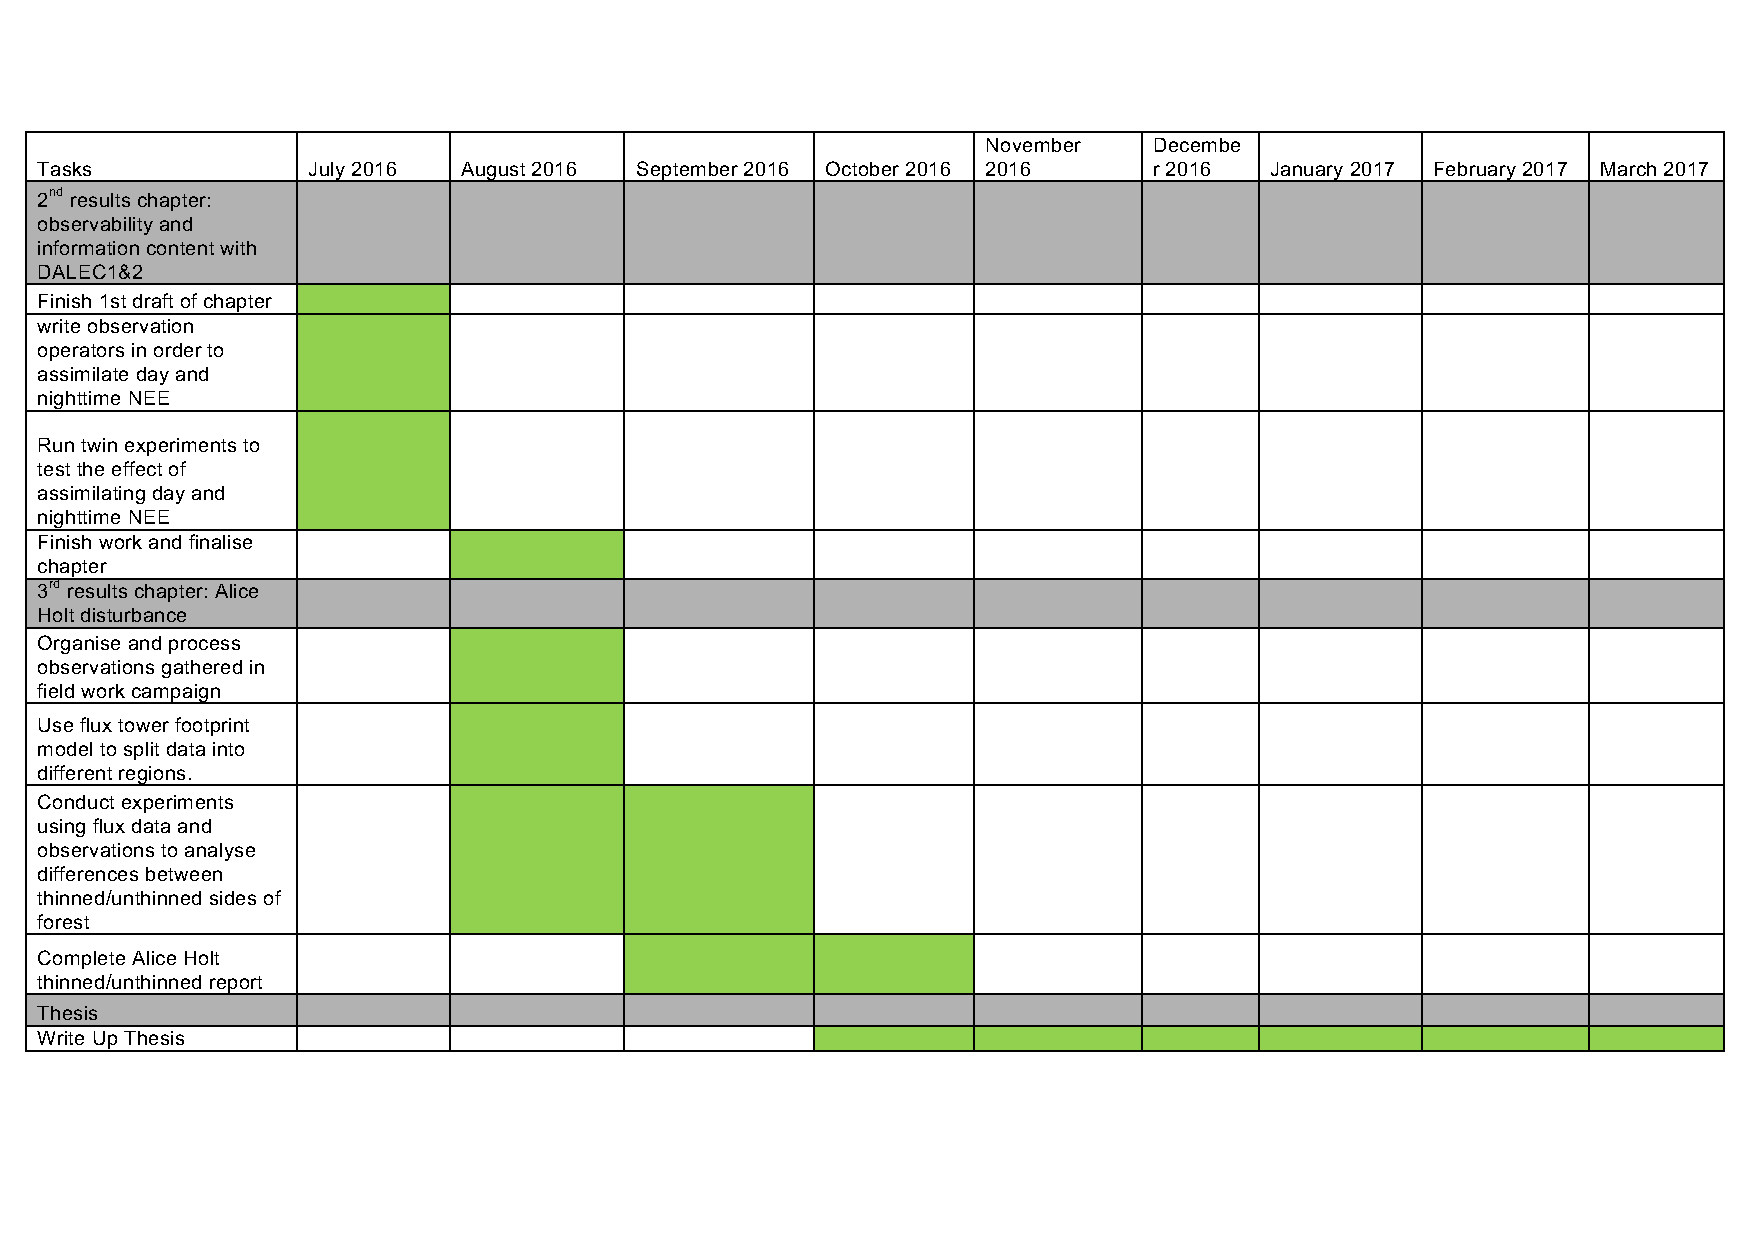
\includegraphics[width=1.\textwidth]{Tasks.pdf}
    \caption{Gantt chart for remaining work to be completed.}
    \label{fig:PropProf}
\end{sidewaysfigure}

\end{document}